\chapter{Wstęp}

\section{Cel projektu}

Celem projektu jest stworzenie aplikacji webowej do zleceń dla transportów okazjonalnych, która zoptymalizuje procesy logistyczne i wyeliminuje nieefektywne wykorzystanie zasobów transportowych. Aplikacja umożliwi użytkownikom łatwe i szybkie znalezienie odpowiedniego przewoźnika lub zleceniodawcy, co spowoduje redukcje pustych przebiegów i tym samym kosztów transportu.
Główne cele projektu:
\begin{enumerate}
\item Optymalizacja procesów logistycznych: Poprzez automatyzację procesu wyszukiwania i dopasowywania zleceń transportowych, aplikacja usprawni komunikację między zleceniodawcami a przewoźnikami, skracając czas potrzebny na znalezienie odpowiedniego transportu.
\item Eliminacja pustych przebiegów: Aplikacja umożliwi przewoźnikom znalezienie ładunków na trasach powrotnych, co zmniejszy liczbę pustych przebiegów i przyczyni się do oszczędności paliwa, co zredukuje koszty.
\item Redukcja kosztów transportu: Dzięki lepszemu dopasowaniu potencjalnych kontrahentów dla usług transportowych, aplikacja pozwoli na obniżenie kosztów transportu zarówno dla zleceniodawców, jak i przewoźników.
\item Poprawa bezpieczeństwa i jakości usług: Aplikacja umożliwi weryfikację kwalifikacji przewoźników oraz ocenę jakości świadczonych usług, co przyczyni się do zwiększenia bezpieczeństwa i zadowolenia klientów.
\item Ułatwienie dostępu do rynku transportowego: Aplikacja stworzy platformę, która ułatwi zarówno doświadczonym przewoźnikom, jak i nowym podmiotom na rynku. 
\end{enumerate}
Realizacja tych celów przyczyni się do stworzenia nowoczesnej i efektywnej aplikacji, która wspomoże rynek zleceń transportowych, przynosząc korzyści zarówno dla zleceniodawców, jak i przewoźników.

\section{Transport okazjonalny}

Transport okazjonalny to przewóz towarów, który nie spełnia definicji przewozu regularnego. Oznacza to, że odbywa się on bez ustalonego z góry rozkładu jazdy i może dotyczyć zarówno tras krajowych, jak i międzynarodowych. Pojazdy wykonują swoje trasy w zależności od zapotrzebowania klientów. Sam przewóz zaś zlecany jest na potrzebę klienta, nie określna on jednak, dokładnego terminu odbycia trasy.

\section{Wymagania aplikacji}
Wymagania funkcjonalne
\begin{enumerate}
\item Uwierzytelnianie: Aplikacja będzie wykorzystywała system rejestracj oraz logowania. W serwisie weryfikacją użytkowników zajmować się będzie moderator.
\item System rekomendacji: Podczas wprowadzania danych o trasie, użytkownik będzie informowany o dostępnych zleceniach dodanych przez innych użytkowników.
\item Dodawanie ogłoszeń: system powinien pozwalać użytkownikom, na dodawanie publicznych informacji o planowanych przez siebie trasach oraz zleceniach transportowych.
\item Komunikacja między użytkownikami: Jednym z założeń projektowych jest dodanie możliwości korespondencji przez czat tekstowy między zleceniodawcami, a przewoźnikami, bezpośrednio w aplikacji.
\item Podpisywanie umowy: użytkownicy, po negocjacji warunków umowy, otrzymają wygenerowany przez serwis dokument finalizujący transakcje.
\item System potwierdzania kwalifikacji: aplikacja, chcąc zachować maksymalne bezpieczeństwo użytkowników, będzie wymagać potwierdzania kwalifikacji przewoźników. Aby kwalifikacja mogła się wyświetlać na profilu przewoźnika, potrzebna jest weryfikacja uprawnień przeprowadzana przez moderatorów serwisu.
\item Weryfikacja dodawanych ogłoszeń: zanim ogłoszenie wyświetlać się będzie dla wszystkich użytkowników, wymagana będzie akceptacja jednego z moderatorów serwisu.
\end{enumerate}
Wymagania niefunkcjonalne
\begin{enumerate}
\item Innowacyjność: Wykorzystanie nowoczesnych technologii, takich jak \texttt{TypeScript}, \texttt{Next.js}, \texttt{Tailwind CSS}, \texttt{Node.js} oraz \texttt{PostgreSQL}, zapewni wysoką wydajność, skalowalność i bezpieczeństwo aplikacji.
\item Intuicyjny interfejs użytkownika: Aplikacja będzie posiadać prosty i intuicyjny interfejs użytkownika, który umożliwi łatwą obsługę zarówno dla zleceniodawców, jak i przewoźników.
\item Dostępność na różnych urządzeniach: Aplikacja będzie responsywna i dostosowana do różnych urządzeń, takich jak komputery, tablety i smartfony, co zapewni wygodę użytkowania w dowolnym miejscu i czasie.
\item Wielojęzyczność: Użytkownicy korzystający z aplikacji, będą mieli możliwość wyboru jednego z trzech przewidzianych języków: polski, angielski oraz niemiecki. Co przełoży się na międzynarodowy aspekt aplikacji.
\item Graficzne przedstawienie trasy: w ogłoszeniach dodanych przez użytkowników, wyświetlana będzie mapa z zaznaczoną trasą. Ułatwi to użytkownikom zobrazowanie planowanego kursu.
\end{enumerate}

\section{Przypadki użycia}
Idnetyfikacja aktorów:

\begin{enumerate}
\item Użytkownik - ogólny użytkownik systemu. Reprezentuje dowolną osobę korzystającą z serwisu, jego przypadki użycia będą dziedziczone przez wszystkich innych aktorów systemu.
\item Przewoźnik - aktor odpowiedzialny za transport towarów. Przewoźnik może aktualizować swoje kwalifikacje, przeglądać dostępne zlecenia, dodawać ogłoszenia o planowanych trasach, komunikować się z autorami ogłoszeń, przyjmować zlecenia oraz oceniać i komentować kontrahentów.
\item Zleceniodawca - użytkownik systemu, który zleca transport towarów. Może dodawać nowe zlecenia transportowe, podobnie jak przewoźnik, może również przeglądać ogłoszenia przewoźników oraz komunikować się z autorami ogłoszeń.
\item Moderator - osoba odpowiedzialna za zarządzanie systemem. Moderator potwierdza kwalifikacje przewoźników, zatwierdza lub usuwa nowe ogłoszenia i zlecenia oraz blokuje konta użytkowników.
\item Administrator - użytkownik umiejscowiony najwyżej w hierarhii systemu. Może on wykonywać wszystko co moderator, lecz ma również możliwość dodawania nowych moderatorów lub usuwania obecnych.
\end{enumerate}

\begin{figure}[H]
	\centering
		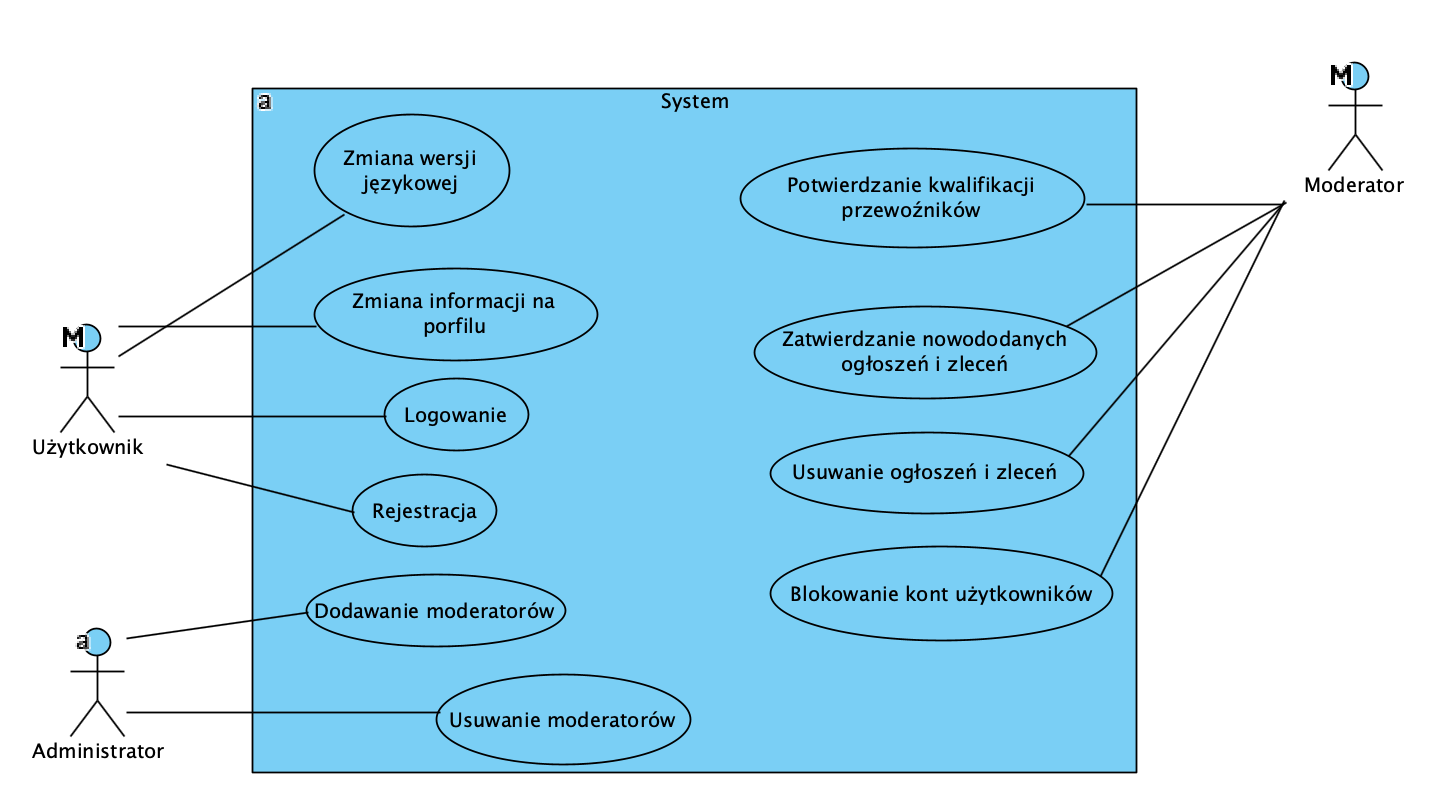
\includegraphics[width=0.9\linewidth]{rozdzial1/ogolny_schemat.png}
	\caption{Diagram głownych funkcjonalności aplikacji}
	\label{Rys. fig:Diagram głownych funkcjonalności aplikacji}
\end{figure}

Na powyższym obrazku przedstawiony został diagram przypadków użycia dla przewoźnika oraz zleceniodawcy. 

\begin{figure}[H]
	\centering
		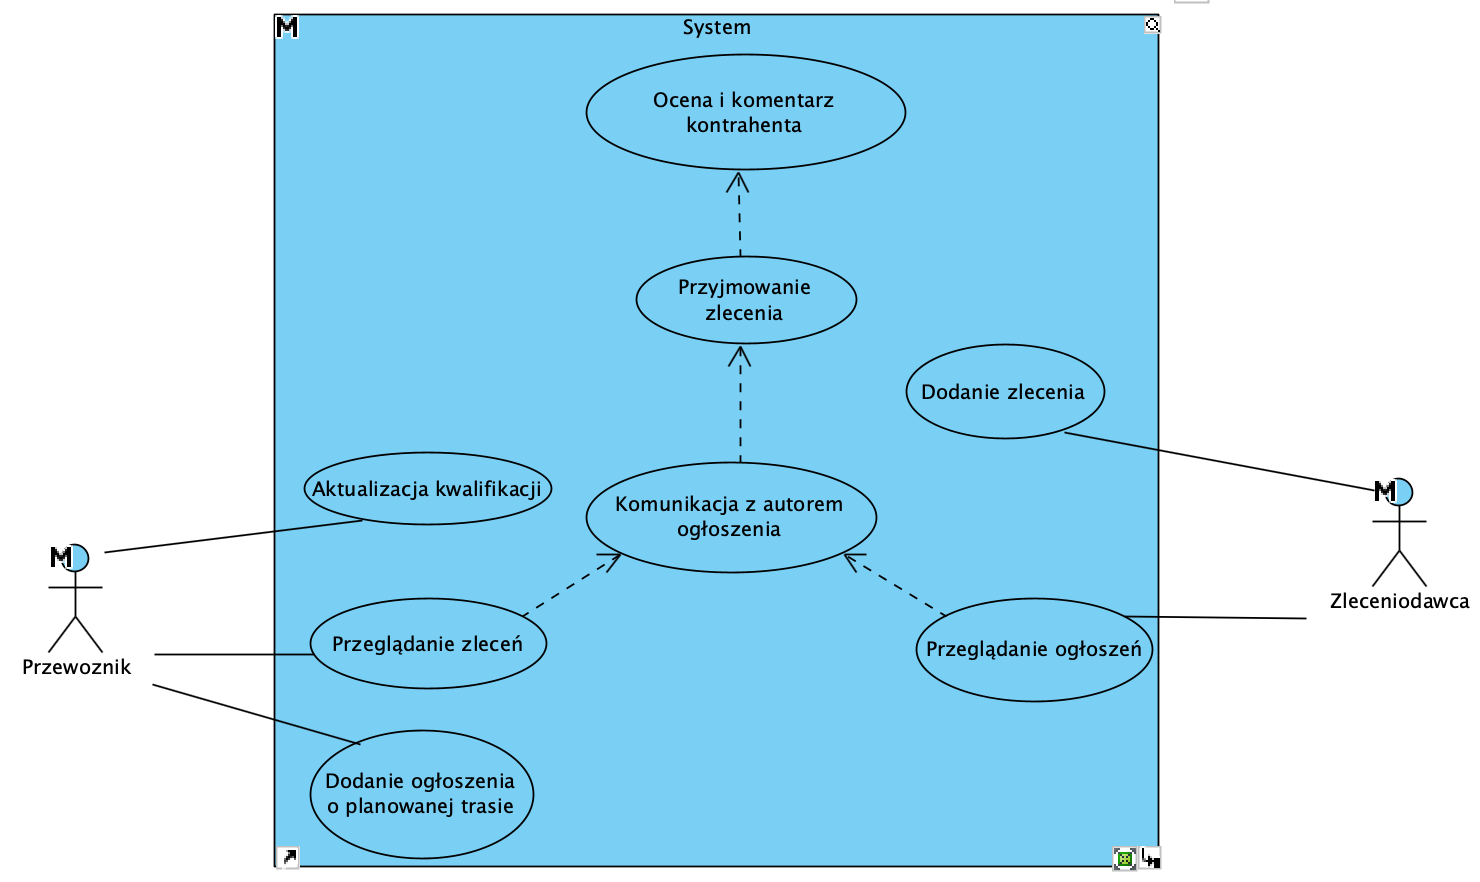
\includegraphics[width=0.9\linewidth]{rozdzial1/glowne_zalozenia.png}
	\caption{Główne założenia projektowe od strony zarządzania serwisem}
	\label{Rys. fig:Główne założenia projektowe od strony zarządzania serwisem}
\end{figure}

Diagram ukazujący główne założenia systemu od strony zarządzania serwisem, w tym możliwości użytkownika, moderatora oraz administratora.

\begin{figure}[H]
	\centering
		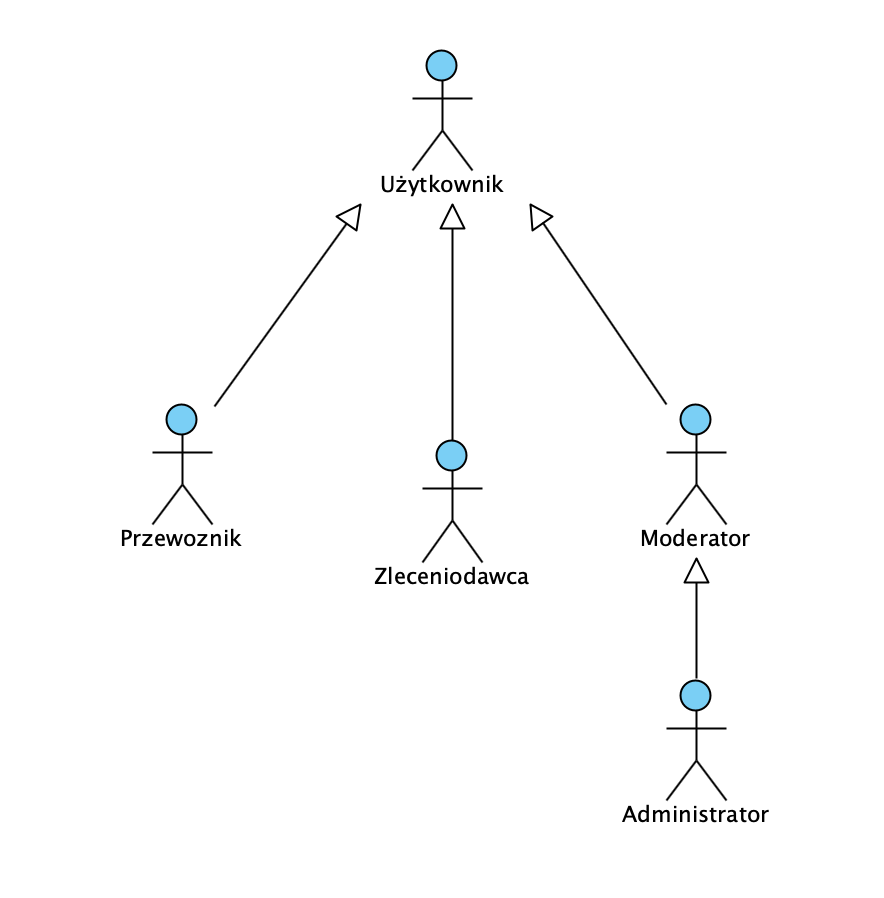
\includegraphics[width=0.6\linewidth]{rozdzial1/dziedziczenie.png}
	\caption{Graficzne ukazanie dziedziczenia możliwości aktorów}
	\label{Rys. fig:Graficzne ukazanie dziedziczenia możliwości aktorów}
\end{figure}

Wszyscy aktorzy systemu, będą dziedziczyć przypadki użycia od użytkownika, co zostało przedstawione graficznie powyżej.